\documentclass[10pt]{article}
\usepackage[margin=1in]{geometry}
\usepackage{booktabs,graphicx,amsmath,siunitx}
\usepackage[hidelinks]{hyperref}
\title{Supplementary Material: Extensive Ablation Study of Hamiltonian--Geometric Optimization}
\author{Reproducible computational supplement}
\date{Generated 2026-07-20 21:33:55 +0530}
\begin{document}\maketitle
\section{Scope and claims}
This supplement reports raw multi-seed ablations generated by
\texttt{run\_ablation\_study.py}.  Paired initializations are retained across
configurations.  The exact full-matrix architecture is evaluated only where
its parameter-dependent metric and finite-difference forces are tractable.
The CUDA study evaluates the documented diagonal reduction and is labeled
accordingly.  No missing GPU run is presented as completed.

\section{Experimental design}
The architecture experiment crosses geometric force ($G$), memory force
($M$), and spectral-entropy force ($S$) in a complete $2^3$ factorial under a
curvature-derived Hessian metric and an unrelated positive-definite control
metric.  The chaotic quantum experiment repeats the same eight configurations
with paired problem seeds and adds AdamW, heavy-ball, and entropy-descent
references.  Medians and nonparametric bootstrap 95\% intervals use raw
per-seed values.  Diverged trials remain in the raw CSV and are counted.

\section{Full-architecture factorial results}
\begin{table}[ht]\centering\scriptsize
\begin{tabular}{llrrrr}\toprule
Metric & Config. & $n$ & Median loss & 95\% CI & Diverged \\\midrule
control & G0M0S0 & 40 & -25.24 & [-33.2, -19.39] & 0 \\
control & G0M0S1 & 40 & -25.24 & [-33.2, -19.39] & 0 \\
control & G0M1S0 & 40 & -25.29 & [-33.2, -19.39] & 0 \\
control & G0M1S1 & 40 & -25.29 & [-33.2, -19.39] & 0 \\
control & G1M0S0 & 40 & -25.24 & [-33.2, -19.39] & 0 \\
control & G1M0S1 & 40 & -25.24 & [-33.2, -19.39] & 0 \\
control & G1M1S0 & 40 & -25.29 & [-33.2, -19.39] & 0 \\
control & G1M1S1 & 40 & -25.29 & [-33.2, -19.39] & 0 \\
hessian & G0M0S0 & 40 & -33.2 & [-33.2, -25.29] & 0 \\
hessian & G0M0S1 & 40 & -33.2 & [-33.2, -25.29] & 0 \\
hessian & G0M1S0 & 40 & -33.2 & [-33.2, -25.29] & 0 \\
hessian & G0M1S1 & 40 & -33.2 & [-33.2, -25.29] & 0 \\
hessian & G1M0S0 & 40 & -33.2 & [-33.2, -25.29] & 0 \\
hessian & G1M0S1 & 40 & -33.2 & [-33.2, -25.29] & 0 \\
hessian & G1M1S0 & 40 & -33.2 & [-33.2, -25.29] & 0 \\
hessian & G1M1S1 & 40 & -33.2 & [-33.2, -25.29] & 0 \\
\bottomrule\end{tabular}
\caption{Paired multi-seed full-architecture results.}
\end{table}
\begin{figure}[ht]\centering
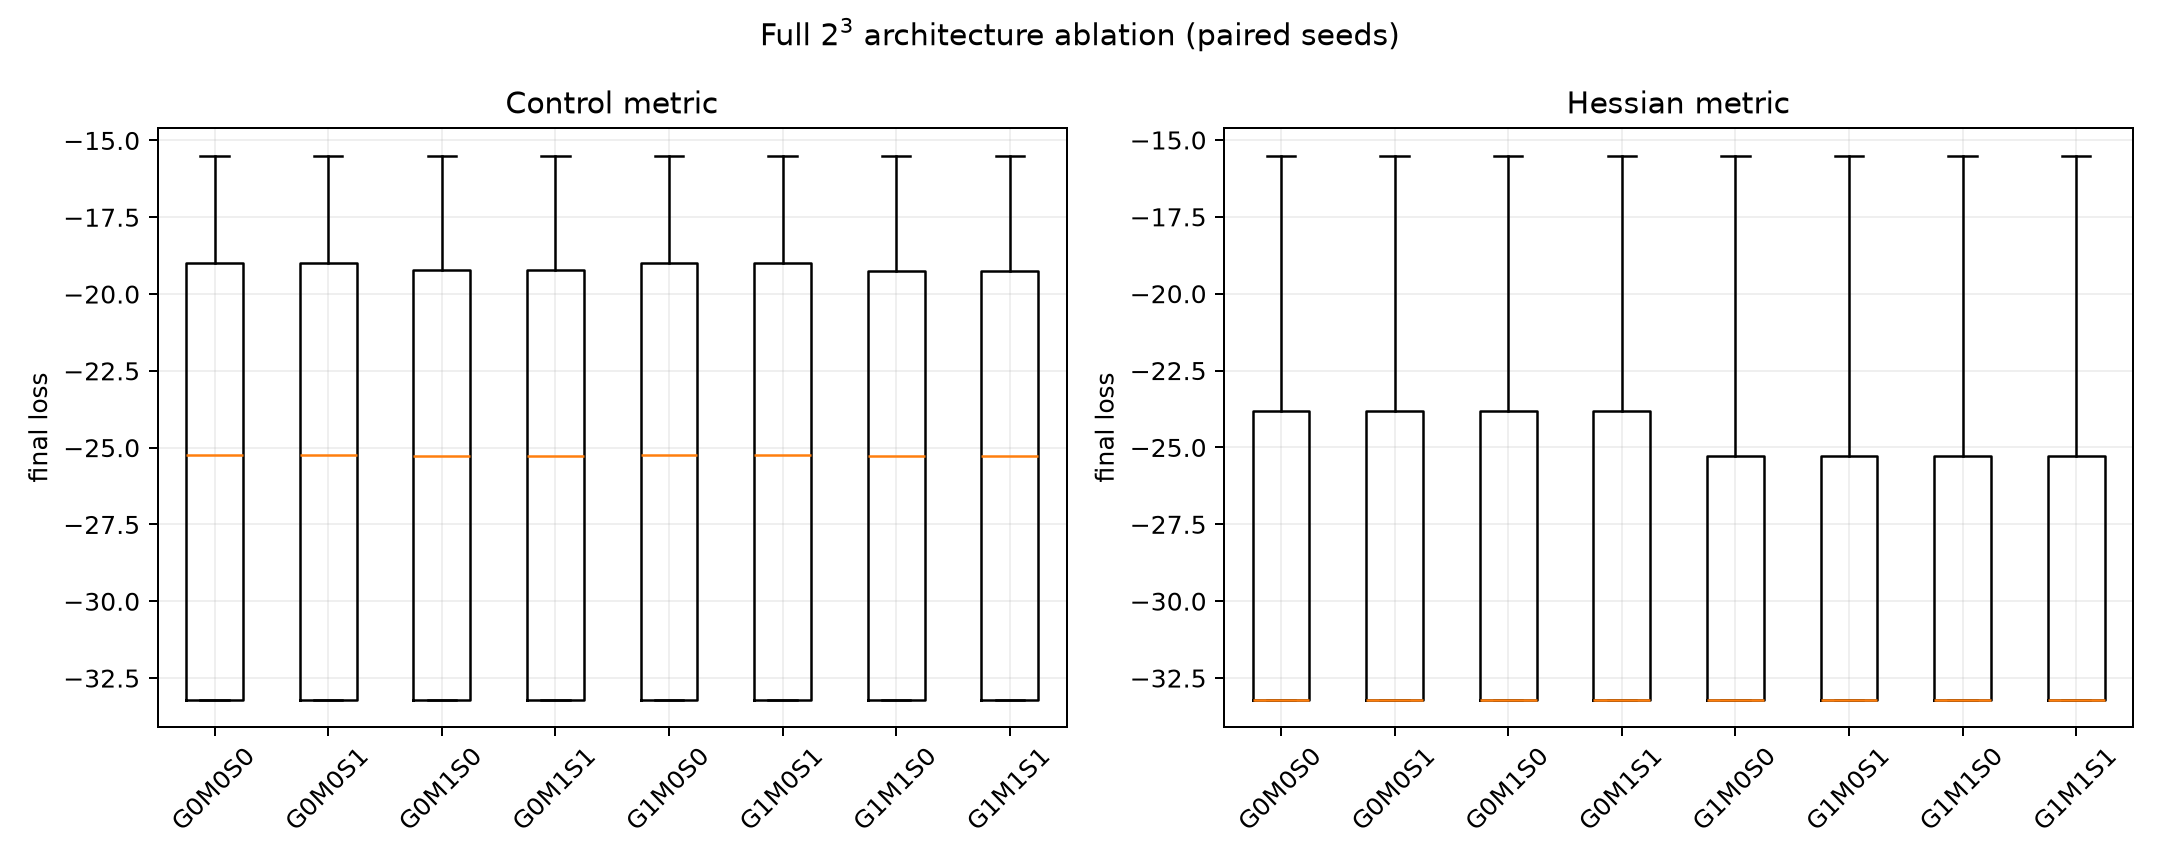
\includegraphics[width=.95\linewidth]{figures/architecture_factorial.png}
\caption{Final-loss distributions for the complete factorial.}
\end{figure}

\section{Factorial effect estimates}
Effects are twice the $\pm1$-coded OLS coefficient on
$\log_{10}(L-L_{\min}+10^{-10})$.  They measure association within this
controlled design, not universal optimizer superiority.
\begin{table}[ht]\centering\small
\begin{tabular}{llrr}\toprule
Study/metric & Factor & Effect & $p$ \\\midrule
architecture/control & G & -0.00527 & 0.991 \\
architecture/control & M & -0.485 & 0.304 \\
architecture/control & S & 0.585 & 0.216 \\
architecture/hessian & G & -0.321 & 0.541 \\
architecture/hessian & M & 0.189 & 0.719 \\
architecture/hessian & S & 2.08 & 9.25e-05 \\
quantum/quantum & G & 2.63 & 4.89e-16 \\
quantum/quantum & M & -2.03 & 6.33e-16 \\
quantum/quantum & S & -1.88 & 6.86e-16 \\
\bottomrule\end{tabular}
\caption{Main factorial effects. Full interactions and standard errors are in \texttt{results/factorial\_effects.csv}.}
\end{table}

\section{Chaotic quantum-control replication}
\begin{table}[ht]\centering\small
\begin{tabular}{lrrrr}\toprule
Configuration & $n$ & Fidelity & 95\% CI & Runtime (s) \\\midrule
G0M0S0 & 1 & 0.4160 & [0.4160, 0.4160] & 0.745 \\
G0M0S1 & 1 & 0.4194 & [0.4194, 0.4194] & 7.688 \\
G0M1S0 & 1 & 0.4225 & [0.4225, 0.4225] & 0.799 \\
G0M1S1 & 1 & 0.4267 & [0.4267, 0.4267] & 7.974 \\
G1M0S0 & 1 & 0.4078 & [0.4078, 0.4078] & 7.853 \\
G1M0S1 & 1 & 0.3792 & [0.3792, 0.3792] & 15.220 \\
G1M1S0 & 1 & 0.3863 & [0.3863, 0.3863] & 8.165 \\
G1M1S1 & 1 & 0.3961 & [0.3961, 0.3961] & 15.529 \\
adamw & 1 & 0.8398 & [0.8398, 0.8398] & 0.288 \\
entropy\_descent & 1 & 0.6384 & [0.6384, 0.6384] & 0.656 \\
heavy\_ball & 1 & 0.7902 & [0.7902, 0.7902] & 0.276 \\
\bottomrule\end{tabular}
\caption{Best-seen fidelity across paired kicked-top problem seeds.}
\end{table}
\begin{figure}[ht]\centering
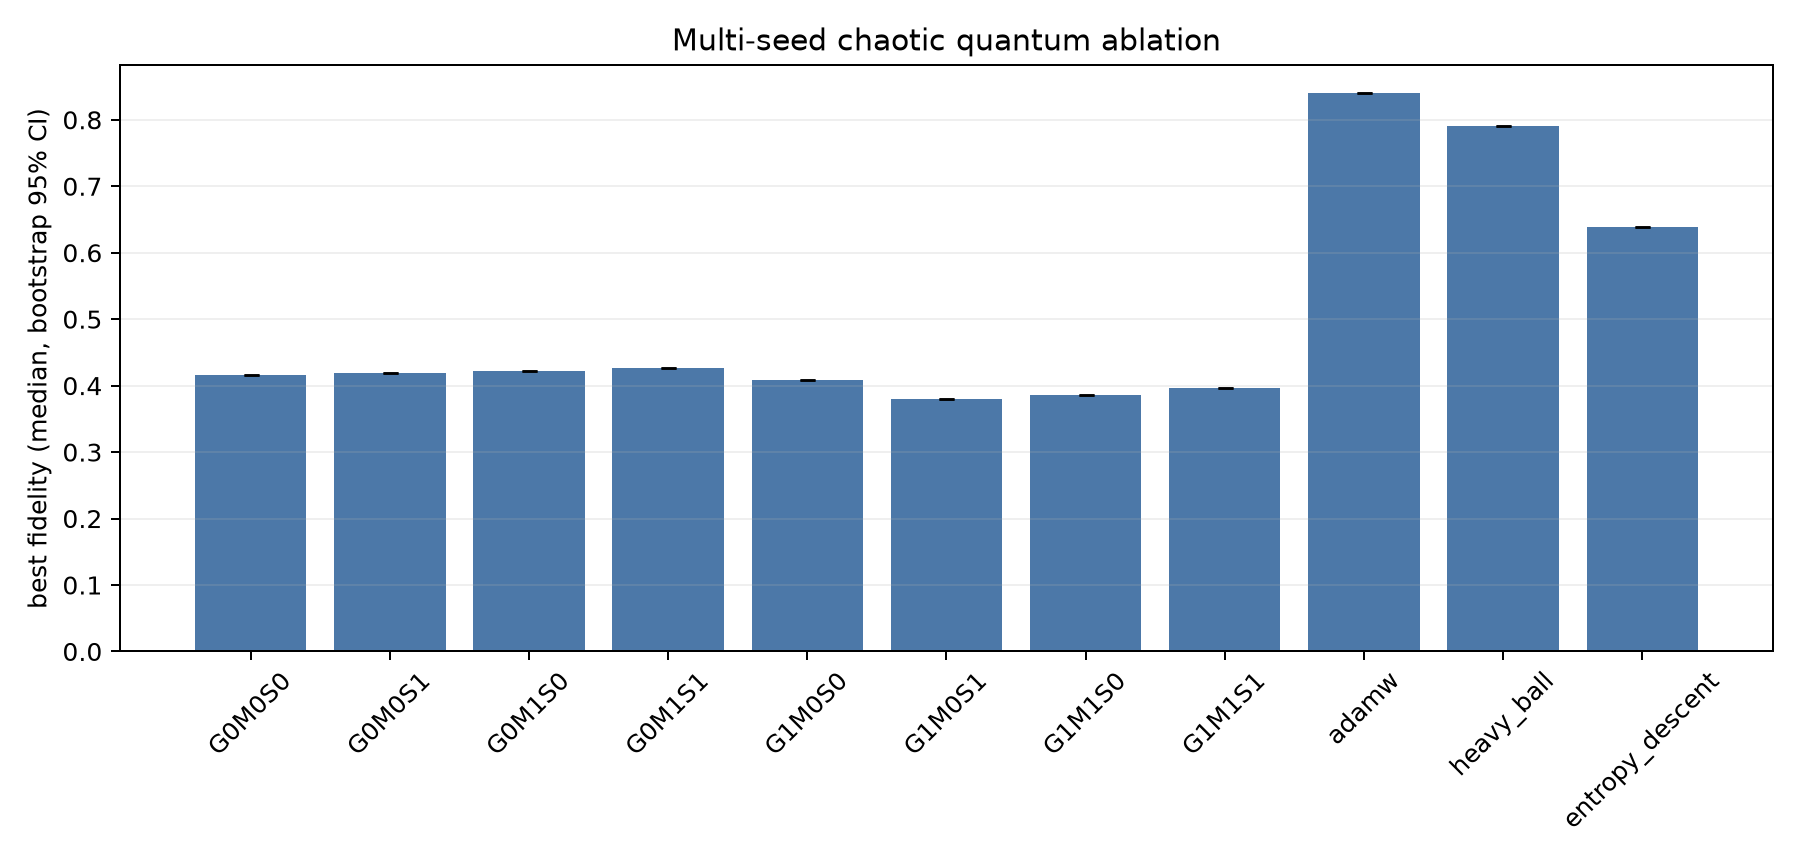
\includegraphics[width=.95\linewidth]{figures/quantum_ablation.png}
\caption{Median quantum fidelity with bootstrap confidence intervals.}
\end{figure}


\section{CUDA neural scaling ablation}
This experiment uses the repository's diagonal-metric Torch reduction; it is
not evidence that a full Hessian or finite-difference geometric force scales
to neural networks.  CUDA execution was verified on
\texttt{NVIDIA GeForce GTX 1050}.
\begin{table}[ht]
\centering\small
\begin{tabular}{lrrrr}\toprule
Configuration & $n$ & Accuracy & 95\% CI & Runtime (s) \\\midrule
AdamW & 2 & 0.8746 & [0.8745, 0.8748] & 0.20 \\
HG\_metric\_momentum & 2 & 0.8253 & [0.8208, 0.8298] & 0.36 \\
HG\_metric\_no\_momentum & 2 & 0.3350 & [0.3008, 0.3691] & 0.28 \\
HG\_scalar\_momentum & 2 & 0.8220 & [0.8091, 0.8350] & 0.25 \\
HG\_scalar\_no\_momentum & 2 & 0.3521 & [0.3330, 0.3711] & 0.28 \\
SGD\_momentum & 2 & 0.4292 & [0.4194, 0.4390] & 0.15 \\
\bottomrule\end{tabular}
\caption{CUDA component-ablation results.}
\end{table}
\begin{figure}[ht]\centering
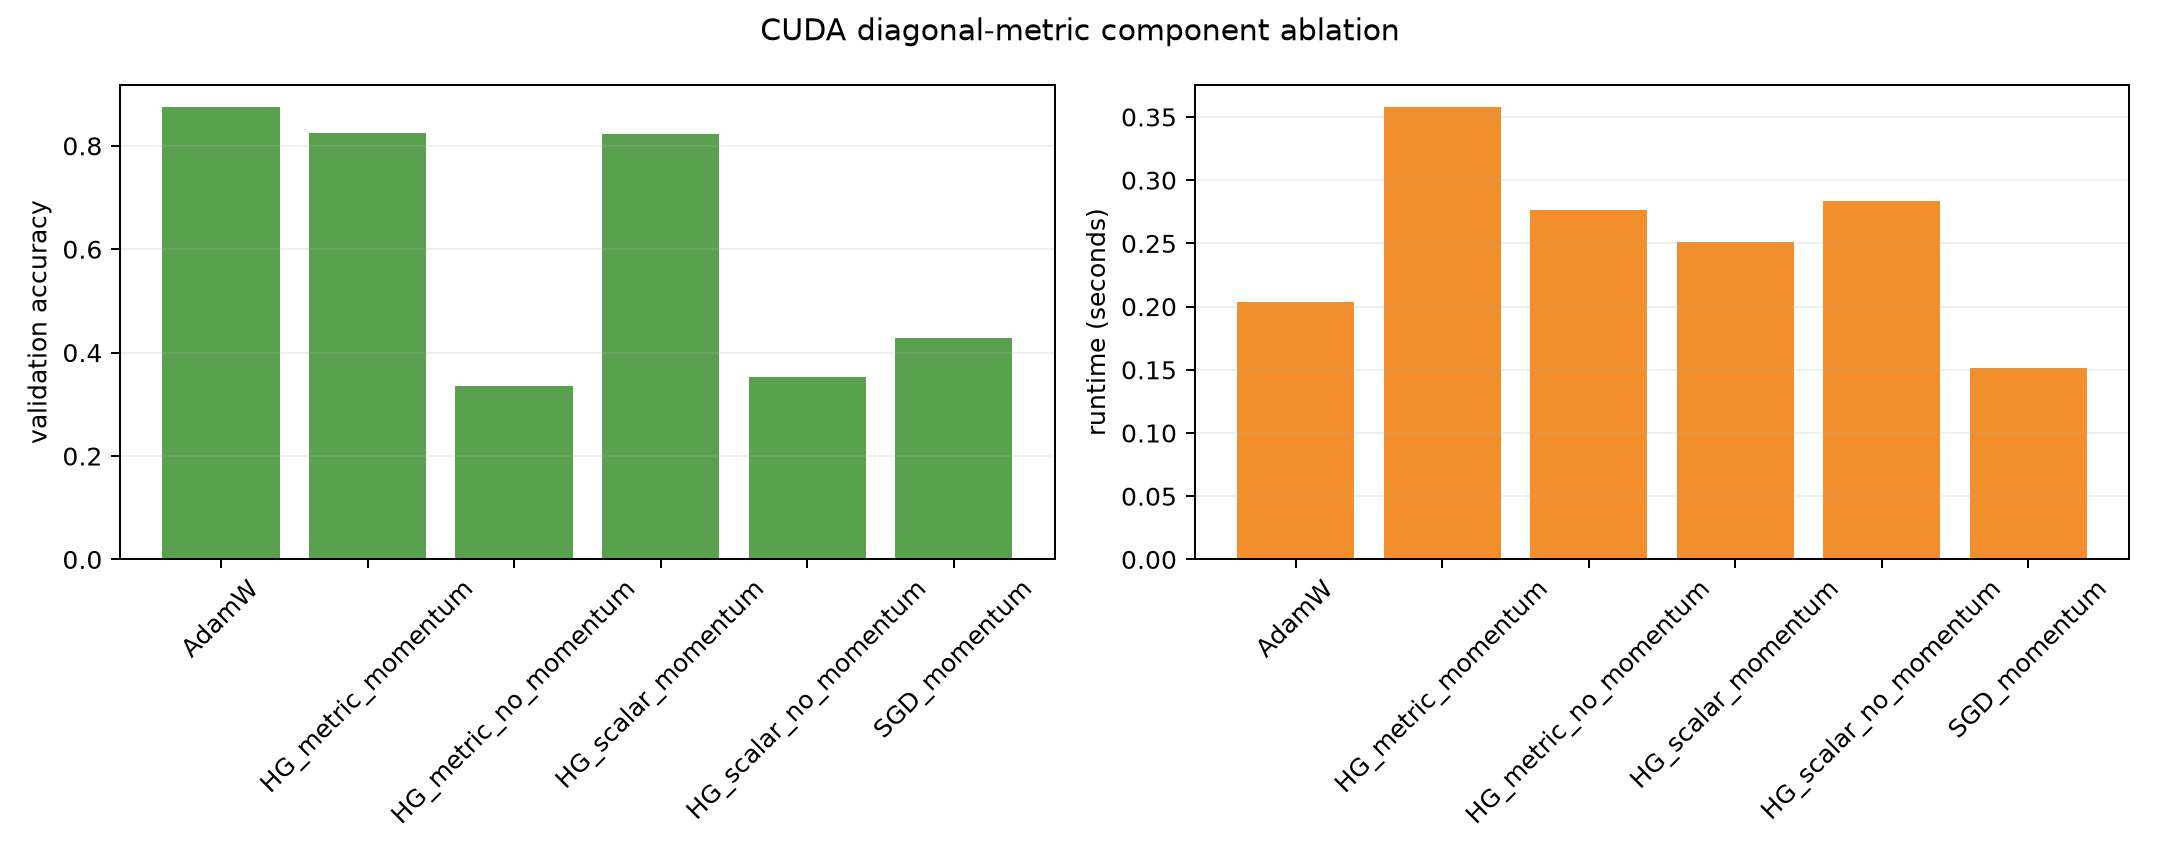
\includegraphics[width=.95\linewidth]{figures/gpu_ablation.png}
\caption{Accuracy and compute cost for the CUDA study.}
\end{figure}

\section{Reproducibility and limitations}
Software and device metadata are stored in \texttt{results/metadata.json}.
Raw observations and histories are retained as CSV files.  Hyperparameters
are fixed before the seed sweep, so these results test robustness of those
settings rather than granting each configuration a different tuning budget.
The quartic task isolates mechanisms but cannot establish application-wide
generalization.  The quantum workload is small, and the CUDA benchmark uses a
diagonal approximation because a dense metric is infeasible at neural-network
scale.  Claims should therefore remain specific to the measured tasks.
\end{document}
